% kompilace xelatex prezentace.tex
% dokumentace k beameru: http://ftp.cvut.cz/tex-archive/macros/latex/contrib/beamer/doc/beameruserguide.pdf

% nastavení formátu prezentace 16:9
\documentclass[czech,aspectratio=169]{beamer}

\usepackage{polyglossia}
\setmainlanguage{czech}

% nastavení vzhledu
% další možnosti vzhledu viz https://hartwork.org/beamer-theme-matrix/
\usetheme{Madrid}
\usecolortheme{whale}
\usepackage{subfig}

% for setting different borders
\usepackage{geometry}

% left, right v includegraphics
\usepackage[export]{adjustbox}

\usepackage{media9} % prehravani videa

% vzhled slajdů vnitřní téma (např. vzhled odrážek)
\useinnertheme{rectangles} %možnosti: default circles rectangles rounded inmargin
% vzhled slajdů vnější téma
\useoutertheme{default} %možnosti: default, miniframes, smoothbars, sidebar, split, shadow, tree, smoothtree, infolines

% zavedeme čvutí modou barvu
\definecolor{CVUT}{HTML}{0065BD}
% čvutí modou použijeme jako hlavní barvu prezentace
\setbeamercolor{structure}{bg=white,fg=CVUT}

% jako font prezentace nadefinujeme oficiální ČVUT písmo Technika -- pokud chcete použít, musíte si font nainstalovat nebo jej nahrát na Overleaf
% https://www.cvut.cz/logo-a-graficky-manual  -- inforek, přihlášení přes celoškolské heslo
%\usepackage{fontspec}
%\setsansfont{Technika-Kniha}

% vypneme navigační panel beamer (pro zapnutí zakomentujeme)
\beamertemplatenavigationsymbolsempty

% vygenerujeme slajdy s poznámkami -- ty si můžete vytisknout a mít je na obhajobu s sebou (pokud zapomenete slova, nebo kdyby nefungovalo promítání z nějakého důvodu)
%\setbeameroption{show notes}

% vygeneruje slajdy s poznámky vhodné pro promítání na dvou monitorech -- na obhajobu nevyužijete
%\usepackage{pgfpages}
%\setbeameroption{show notes on second screen}

% variable block width
\newenvironment<>{varblock}[2][.9\textwidth]{%
	\setlength{\textwidth}{#1}
	\begin{actionenv}#3%
		\def\insertblocktitle{#2}%
		\par%
		\usebeamertemplate{block begin}}
	{\par%
		\usebeamertemplate{block end}%
\end{actionenv}}

% fromat datumu
\usepackage[style=dmyyyy,datesep={.}]{datetime2}

% další balíčky
\usepackage{graphicx}
\usepackage{hyperref}
\usepackage{tikz}
\usetikzlibrary{chains,fit,shapes}

% Údaje o prezentaci
\title[GAN Dissection]{GAN Dissection: Visualizing and Understanding Generative Adversarial Networks}
\institute[FIT CTU]{Faculty of Information Technology \\ Czech Technical University in Prague}
\author[M. Šafránek]{Martin Šafránek}
%\date{\today}
\date{}
\titlegraphic{
\includegraphics[width=.1\textwidth]{../media/logo-cvut}}


\begin{document}

\begin{frame}
	\titlepage
	\note{Nezapomenout pozdravit} %tohle je poznámka, ta na slajdu nebude, ale vygeneruje se vedle něj, pokud odkomentujete příkaz výše -- \setbeameroption{show notes}
\end{frame}


%%%%%%%%%%%%%%%%%%%%%%%%%%%%%%%%%%%%%%%%%%%%%%%%%%%%%%%%%%%%%%%%%%%%%%%%%%%%%%
\section{Introduction}
%%%%%%%%%%%%%%%%%%%%%%%%%%%%%%%%%%%%%%%%%%%%%%%%%%%%%%%%%%%%%%%%%%%%%%%%%%%%%%

\begin{frame}{Parts}
	\begin{itemize}
		\item GAN overview
		\item GAN dissection (paper)
	\end{itemize}

\end{frame}

%%%%%%%%%%%%%%%%%%%%%%%%%%%%%%%%%%%%%%%%%%%%%%%%%%%%%%%%%%%%%%%%%%%%%%%%%%%%%%
\section{GAN introduction}
%%%%%%%%%%%%%%%%%%%%%%%%%%%%%%%%%%%%%%%%%%%%%%%%%%%%%%%%%%%%%%%%%%%%%%%%%%%%%%

\begin{frame}{Adversarial Nets Framework}
	\centering
	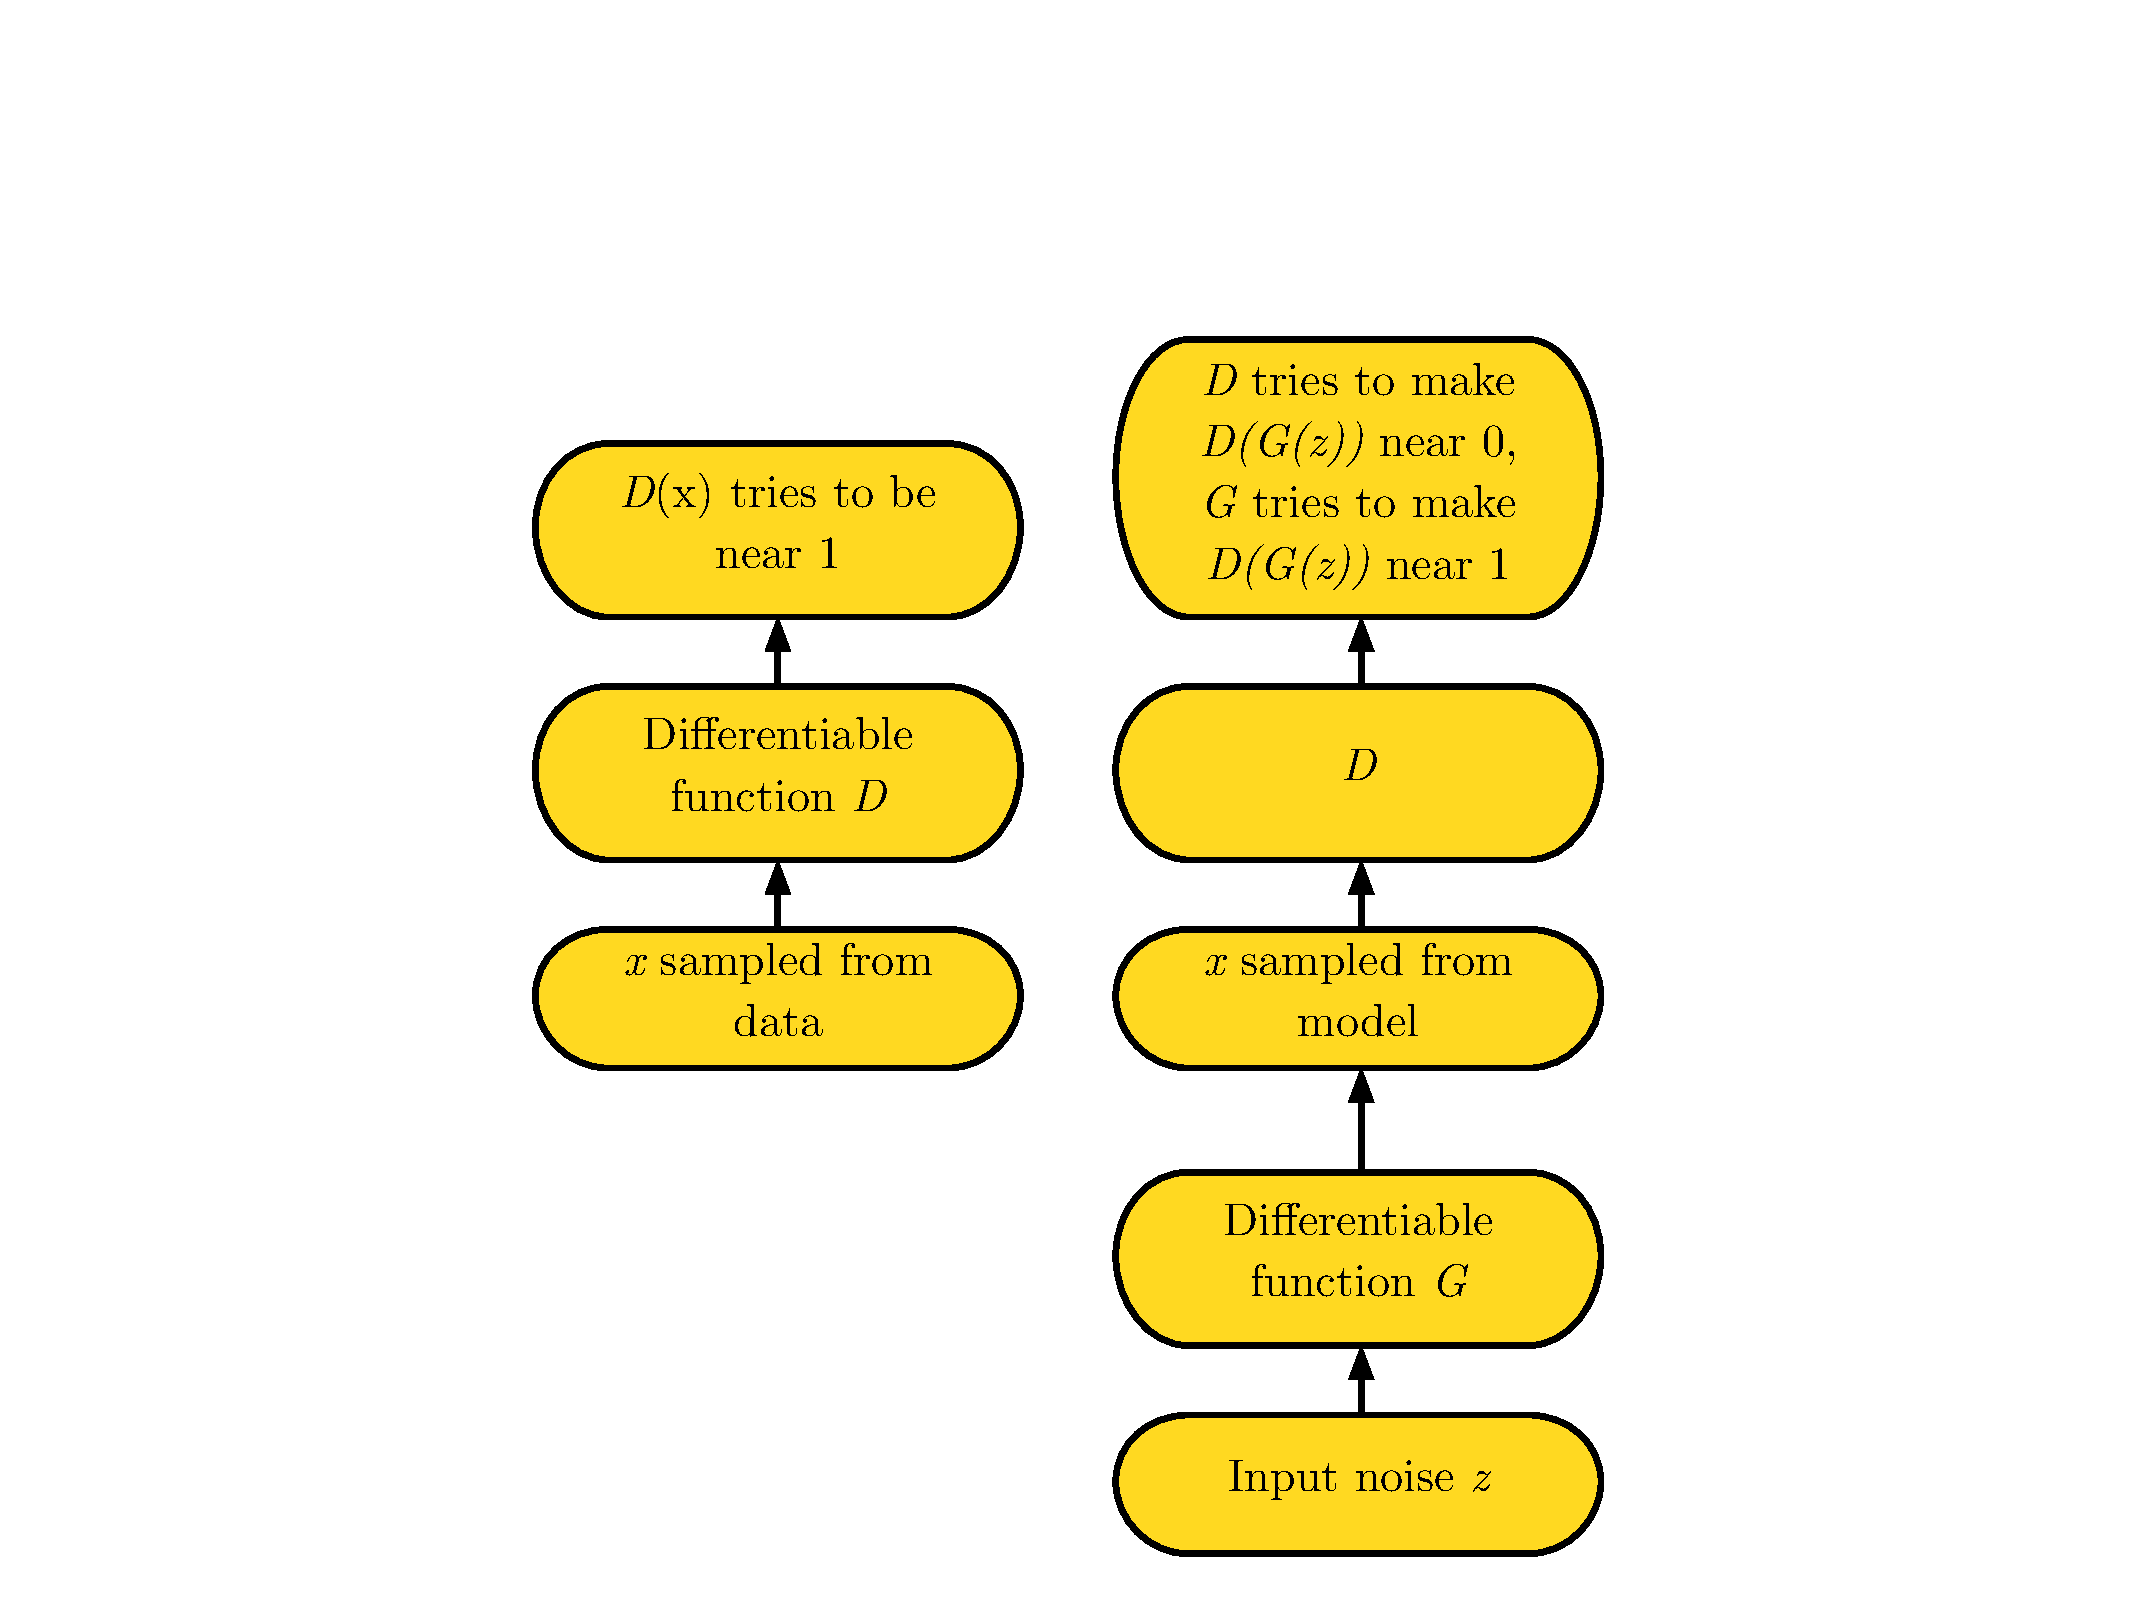
\includegraphics[width=0.8\textheight]{../media/gan_architecture.pdf}
\end{frame}

\begin{frame}{Minimax Game}
	\begin{figure}
		$$
		J^{\left( D \right)} = - \dfrac{1}{2}\mathbb{E}_{x\~{}p_{\rm data}} \, \mathrm{log} \, D(x) - \dfrac{1}{2}\mathbb{E}_z \, \mathrm{log} \, (1-D(G(z)))
		$$
		$$
		J^{G} = -J^{D}
		$$
	\end{figure}
	\begin{itemize}
		\item Generator minimizes the log-probability of the discriminator
		being correct
		\item Equilibrium if the discriminator is unable to differentiate between real and generated input
	\end{itemize}
\end{frame}


%%%%%%%%%%%%%%%%%%%%%%%%%%%%%%%%%%%%%%%%%%%%%%%%%%%%%%%%%%%%%%%%%%%%%%%%%%%%%%
\section{GAN dissection}
%%%%%%%%%%%%%%%%%%%%%%%%%%%%%%%%%%%%%%%%%%%%%%%%%%%%%%%%%%%%%%%%%%%%%%%%%%%%%%

\begin{frame}{The paper}
	\begin{itemize}
		\item presents method for visualizing and understanding GAN
		\item learned GAN contains variables for doors, trees, ...
		\item can interactively manipulate objects in a scene
	\end{itemize}
\end{frame}k


\begin{frame}
	\centering
	\begin{figure}
		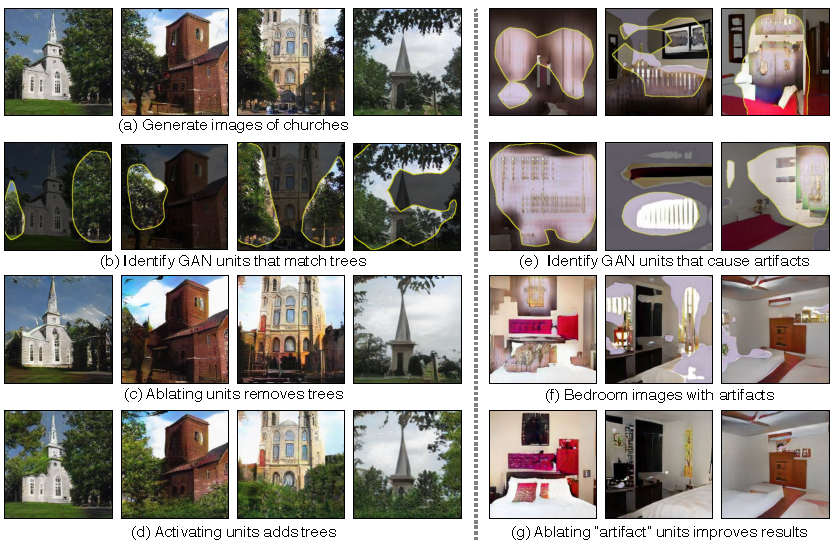
\includegraphics[width=1.3\textheight]{../media/figure_overview}
	\end{figure}
\end{frame}

\begin{frame}{Method}
	\begin{itemize}
		\item
	\end{itemize}
\end{frame}



\end{document}
